\documentclass[dvipdfmx]{beamer}
\usetheme{metropolis}

\title{CTF4y 講義資料}
\date{\today}
\author{yoshiking(@y05h1k1ng)}

\begin{document}
\maketitle

\begin{frame}{問題}
  [TokyoWesterns CTF 4th 2018] Crypto - mixed cipher (233points/39solves)

  いろいろな攻撃手法が一度に学べる!!おいしい!!
\end{frame}

\begin{frame}{やってみそ}
  (スコアサーバーの)8000番が開いてるはず
  \begin{figure}
    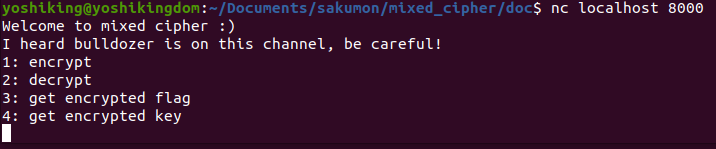
\includegraphics[width=0.8\linewidth]{./img/nc.png}
  \end{figure}
\end{frame}

\begin{frame}{概要}
  4つのメニューがある
  \begin{itemize}
  \item encrypt
  \item decrypt
  \item get encrypted flag
  \item get encrypted key
  \end{itemize}
\end{frame}

\begin{frame}{encrypt}
  入力した値をRSAとAESで暗号化してくれる
  \begin{figure}
    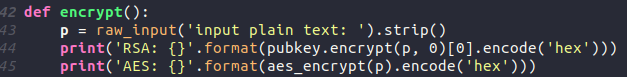
\includegraphics[width=0.8\linewidth]{./img/encrypt.png}
  \end{figure}
\end{frame}

\begin{frame}{decrypt}
  RSAで復号してくれる
  
  ただし、bulldozerが最後の1byte以外を{\bf \#}に置き換える

  $\Rightarrow$ 復号結果の最後の1byteしかわからない!!
  \begin{figure}
    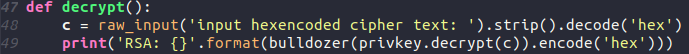
\includegraphics[width=0.8\linewidth]{./img/decrypt.png}
  \end{figure}
\end{frame}

\begin{frame}{get encrypted flag}
  aesで暗号化したflagをくれる

  ただ、ivがわからない({\bf \#}に置き換えられている)
  \begin{figure}
    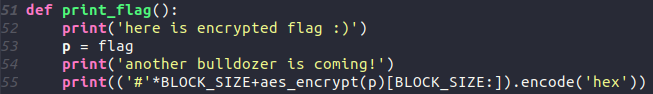
\includegraphics[width=0.8\linewidth]{./img/print_flag.png}
  \end{figure}
\end{frame}

\begin{frame}{get encrypted key}
  RSAで暗号化したaes鍵をくれる
  \begin{figure}
    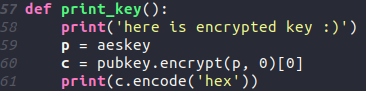
\includegraphics[scale=0.4]{./img/print_key.png}
  \end{figure}
\end{frame}

\begin{frame}{ざっと読んだ感じ...}
  \begin{itemize}
  \item decrypt
    \begin{itemize}
    \item[] 自明にLSB Decryption Oracle Attackですね
    \end{itemize}
  \item get encrypted flag
    \begin{itemize}
    \item[] iv消されてるのどうしようか...
    \end{itemize}
  \end{itemize}
\end{frame}

\section{とりあえずLSB Decryption Oracle Attackやろうぜ!!}

\begin{frame}{LSB Decryption Oracle Attack}
  任意の暗号文を復号した結果の最下位ビットを得ることができるとき、与えられた暗号文に対応する平文を求める攻撃

  \begin{equation}
    2^e * c \equiv (2*m)^e \bmod{n} \nonumber
  \end{equation}
  復号すると、
  \begin{equation}
    (2*m)^{e*d} \equiv 2*m \bmod{n} \nonumber
  \end{equation}
  となり、結果$2*m$について
  \begin{itemize}
  \item 最下位ビットが1であれば、$2*m > n$
  \item 最下位ビットが0であれば、$2*m < n$
  \end{itemize}
\end{frame}

\begin{frame}{もうちょい詳しく...}
  nは奇数
\end{frame}

\begin{frame}{LSB Decryption Oracle Attackでやること}
  \begin{itemize}
  \item print keyで入手できるrsaで暗号化されたaes鍵を復元する
  \end{itemize}
  
  さあ、攻撃!!!の前に...
\end{frame}

\section{$n$持ってないじゃん!!!}

\begin{frame}{$n$の取得}
  \begin{itemize}
  \item これはそんなに難しくない
  \item (LSB Decryption Oracle Attackに比べて)よくやる手法な気がする
  \end{itemize}
\end{frame}

\begin{frame}{$n$の取得}
  encryptで好きな平文を暗号化できる。
  \begin{itemize}
  \item -1を入れるパターンもあるけど、今回は入力できない
  \end{itemize}

  適当な平文$m_i$について、rsaの式をいじってみる。
  \begin{equation}
    m_i ^ e \equiv c_i \bmod{n} \nonumber
  \end{equation}
  より、商と余りの関係から、
  \begin{eqnarray}
    m_i ^ e &=& c_i + k_i * n \nonumber \\
    m_i ^e - c_i &= & k_i * n \nonumber
  \end{eqnarray}
  が求められる。
\end{frame}

\begin{frame}{$n$の取得}
  異なる入力$m_1, m_2$を与えたとき、
  \begin{equation}
    \begin{cases}
      m_1 ^e - c_1 &= k_1 * n \\
      m_2 ^e - c_2 &= k_2 * n
    \end{cases}\nonumber
  \end{equation}
  となる。ここで、この2つの最大公約数を取ると$n$が求めることができる。
  \begin{eqnarray}
    gcd(m_1^e - c_1, m_2^e - c_2) &=& gcd(k_1*n, k_2*n) \nonumber \\
    &=& n \nonumber
  \end{eqnarray}
\end{frame}

\section{とりあえず、$n$の取得、LSB Decryption Oracle Attackまで書いてaes鍵を復元してみよう}

\begin{frame}{現状}
  \begin{itemize}
  \item aes鍵は手に切れた
  \item ただ、ivがない。
  \end{itemize}
\end{frame}

\begin{frame}{ivの入手}
  aes encryptを見てみると、ivの生成はgenrandbitsを使っている
  $Rightarrow$pythonはMersenne Twisterを使ってrandomを生成する...
\end{frame}

\begin{frame}{Mersenne Twister}
\end{frame}

\begin{frame}{Mersenne Twisterの内部状態の復元}
\end{frame}

\end{document}
